\section{Measurable Functions and Integration}

  Now that we've discussed measurability of sets, we need to talk about measurability of functions, and then we can integrate over them.  

\subsection{Measurable Functions}

  \begin{definition}[Measurable Function]
    Given a measurable space $(X, \mathcal{A})$, $f: (X, \mathcal{A}) \longrightarrow \mathbb{R}$ is \textbf{measurable} if 
    \begin{equation}
      f^{-1}(A) \in \mathcal{A} \text{ for all } A \text{ open}
    \end{equation}
    where $f^{-1}(A)$ denotes the preimage of $A$. 
  \end{definition}

  Note that if we take $\mathbb{R}^n$, it can have either its Borel $\sigma$-algebra $\mathcal{B}(\mathbb{R}^n)$ or its Lebesgue $\sigma$-algebra $\mathcal{M}_{\lambda^*}$. Therefore, a function $f: \mathbb{R}^n \longrightarrow \mathbb{R}$ is said to be \textbf{Lebesgue measurable} (\textbf{Borel measurable}) if for every $E \in \mathcal{B}(\mathbb{R})$, $f^{-1}(E) \in \mathcal{M}_{\lambda^*}$ ($f^{-1}(E) \in \mathcal{B}(\mathbb{R}^n)$). Since $\mathcal{B}(\mathbb{R}^n) \subset \mathcal{M}_{\lambda^*}$, all Borel measurable functions are Lebesgue measurable. It follows that any continuous function $f: \mathbb{R}^n \longrightarrow \mathbb{R}$ is Borel (and hence Lebesgue measurable). 


  There are many ways to prove measurability, which we will list below. 

  \begin{theorem}[TFAE]
    The following are equivalent. 
    \begin{enumerate}
      \item $f$ is measurable 
      \item $f^{-1} (U) \in \mathcal{A}$ for all $U \in \mathcal{B}(\mathbb{R}$ 
      \item $f^{-1}((-\infty, t)) \in \mathcal{A} \; \forall t \in \mathbb{R}$. 
    \end{enumerate}
  \end{theorem}

  This immediately implies that monotonic functions on $\mathbb{R}$ are measurable. For example, take $f: [a, b] \longrightarrow \mathbb{R}$ that is nondecreasing. Then, we would like to show that the preimage of every half-interval $(-\infty, t)$ under $f$ is in $\mathcal{B}(\mathbb{R})$. Well if we assume $f(a) \geq t$, then $f(x) > t \; \forall t \in [a, b]$, and so its preimage is $\emptyset$. If $f(a) < t$, having $f(b) < t$ also leads to the preimage being $[a, b]$ (which is the entire space and is in $\mathcal{B}(\mathbb{R})$), and having $f(b) > t$ implies that the preimage is $[a, f^{-1}(t)]$. 

  The following theorem is useful, since we don't want to manually check measurability of every single new function we create. 

  \begin{theorem}[Sloppy Version]
    Given measurable functions $f, g$, the following standard operations on them create new measurable functions: 
    \begin{enumerate}
      \item $f + g$ is measurable 
      \item $f \cdot g$ is measurable 
      \item $\alpha f$ is measurable 
      \item $f / g$ is measurable on $\{x \mid g(x) \neq 0\}$ 
      \item $f \vee g \coloneqq \max (f, g)$ is measurable 
      \item $f \wedge g \coloneqq \min (f, g)$ is measurable 
    \end{enumerate}
  \end{theorem}

  \begin{theorem}
    Given a sequence of measurable functions $f_1, f_2, \ldots$, we have 
    \begin{equation}
      \lim_{k \rightarrow \infty} f_k
    \end{equation}
    is measurable where it exists. 
  \end{theorem}

\subsection{Simple Functions}

  Remember that Riemann integration is characterized by the approximation of step functions, which are the "building blocks" of Riemann integrable functions. To define the Lebesgue integral, we will consider a generalization of step functions called \textit{simple functions}. A function will be Lebesgue integrable if it can be approximated by these simple functions in some appropriate way. 

  \begin{definition}[Simple Functions]
    For $A \subset X$ (any subset, not just in some $\sigma$-algebra), the \textbf{characteristic}, or \textbf{indicator} \textbf{function} of $A$ is the function $\chi_A : X \longrightarrow \mathbb{R}$ defined 
    \begin{equation}
      \chi_A (x) = \begin{cases} 1 & \text{ if } x \in A \\ 0 & \text{ if else} \end{cases}
    \end{equation}
    A function $\phi: \mathbb{R} \longrightarrow \mathbb{R}$ is called a \textbf{simple function} if it is a finite linear combination of characteristic functions. 
    \begin{equation}
      \phi = \sum_{i=1}^n a_i \chi_{A_i}
    \end{equation}
  \end{definition}

  \begin{lemma}[Measurability on Simple Functions]
    Now, let $(X, \mathcal{A})$ be a measurable space. Then, 
    \begin{equation}
      \phi = \sum_{i=1}^n a_i \chi_{A_i} : (X, \mathcal{A}) \longrightarrow \mathbb{R}
    \end{equation}
    is measurable if all $A_i$ are measurable, i.e. $A_i \in \mathcal{A}$ for all $i$. 
  \end{lemma}
  \begin{proof}
    Let $T$ be an open set in $\mathbb{R}$. Then, for characteristic function $\chi_A$, 
    \begin{equation}
      \chi_A^{-1} (T) = \begin{cases} 
      \emptyset & \text{ if } 0, 1 \not\in T \\
      A & \text{ if } 1 \in T, 0 \not\in T \\
      X \setminus A & \text{ if } 0 \in T, 1 \not\in T \\
      X & \text{ if } 0, 1 \in T
      \end{cases}
    \end{equation}
    and so $\chi_A$ must be measurable if $A \in \mathcal{A}$ (which also by definition implies that $A^c = X \setminus A \in \mathcal{A}$). If $\chi_{A_i}$ is measurable, then the linear combination of measurable functions is also measurable. 
  \end{proof}

  Also observe that the coefficients need not be unique, since we can write 
  \begin{equation}
    1 \cdot \chi_{[0, 1]} + 1 \cdot \chi_{[0.5, 1]} = 1 \cdot \chi_{[0, 0.5]} + 2 \cdot \chi_{[0.5, 1]}
  \end{equation}
  If the $E_i$'s are disjoint, then this decomposition is unique and is called the \textbf{standard representation} of $\phi$. 

  \begin{example}[Step Function as Simple Function]
    For $a, b \in \mathbb{R}$, with $a < b$, let $f: [a, b] \longrightarrow \mathbb{R}$ be a step function. That is, there exists a partition $a = x_0 < x_1 < \ldots < x_n = b$ and constants $c_1, c_2, \ldots, c_n \in \mathbb{R}$ s.t. $f(x) = c_i$ for all $x \in (x_{i-1}, x_i)$ and each $i = 1, \ldots, n$. Then, $f$ is equal to the following simple function, taken over all open intervals and the points $x_j$ at the boundary of each interval. 
    \begin{equation}
      f = \sum_{i=1}^n c_i \chi_{(x_{i-1}, x_i)} + \sum_{j=0}^n f(x_j) \chi_{\{x_j\}}
    \end{equation}
    If we ignore the behavior of $f$ on the partition points $x_j$'s, then $f$ agrees almost everywhere with the simple function 
    \begin{equation}
      \sum_{i=1}^n c_i \chi_{(x_{i-1}, x_i)}
    \end{equation}
  \end{example}

  If the $A_i$'s above are just intervals in $\mathbb{R}$, then $\phi$ reduces to a step function. But the entire problem with intervals is that they are too coarse. We can't work with them, so we generalize them to all measurable sets in $(X, \mathcal{A})$. The Riemann integral is built on an approximation scheme of a function, which we usually want to be continuous to satisfy this approximation, and so, if we want to build an approximation scheme for Lebesgue integrals, we want a similar scheme, i.e. if we take a sequence of simple measurable functions, I can get arbitrarily close to any measurable function $f$. This is exactly what we show below. 

  \begin{theorem}
    If $f: (X, \mathcal{A}) \longrightarrow [0, \infty]$ is measurable, there are simple measurable functions $f_k : (X, \mathcal{A}) \longrightarrow [0, \infty)$ s.t. 
    \begin{equation}
      f_k \leq f_{k+1} \text{ and } f = \lim_{k \rightarrow \infty} f_k
    \end{equation}
    where the inequalities and limits are pointwise. 
  \end{theorem}
  \begin{proof}
    We give a general picture of this proof for a function $f: \mathbb{R} \longrightarrow [0, \infty]$. We can first divide the codomain of the graph below into segments of $t = 1, 2, \ldots$, and take the preimage of all these units under $f$ to get $f_1$. More specifically, $A_1^t = f^{-1} ([t, \infty])$ for all $t$. By measurability of $f$, $A_1^t$ is measurable, and we can assign $f_1 = \chi_{A^1_1} + \chi_{A_1^2} \leq f$. 
    \begin{center}
        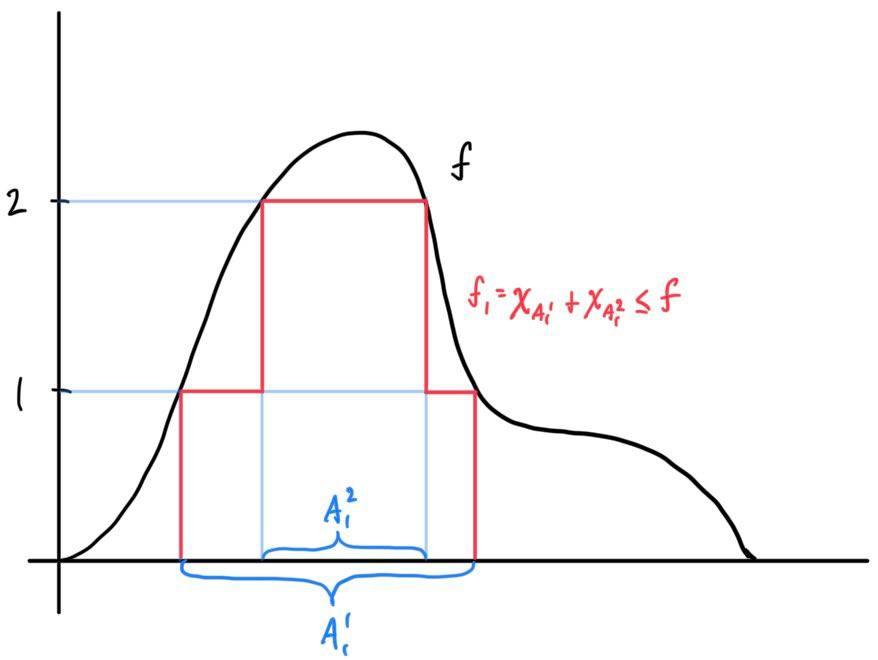
\includegraphics[scale=0.23]{img/Lebesgue_1.jpg}
    \end{center}
    Doing this again with finer subintervals of the codomain gives us, with $f_2 = \chi_{A_2^1} + \chi_{A_2^2} + \chi_{A_2^3} + \chi_{A_2^4} \leq f$. 
    \begin{center}
        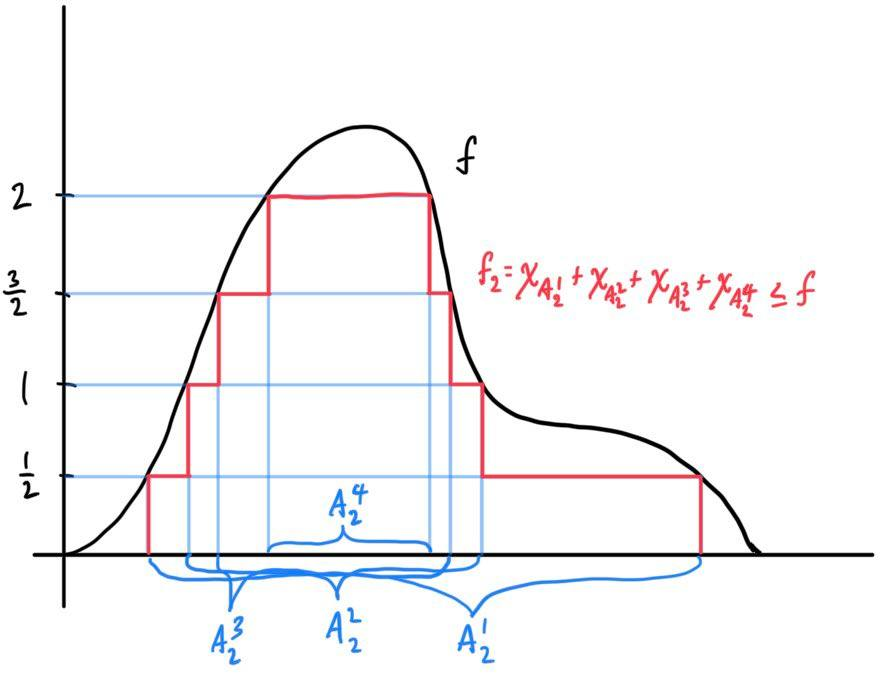
\includegraphics[scale=0.23]{img/Lebesgue_2.jpg}
    \end{center}
    and in general, we have $f_k = \sum_{j=1}^\infty \frac{1}{2^{k-1}} \chi_{A^j_k}$. But we said a simple function is a \textit{finite} sum, and if $\infty$ is in the range of $f$, then this becomes a problem. We can quickly fix this by just truncating the summation at a certain point in the codomain ($f_1$ only considers intervals up to $1$, $f_2$ up to $2$ and so on), ultimately giving us 
    \begin{equation}
      f_k = \sum_{j=1}^{k 2^{k-1}} \frac{1}{2^{k-1}} \chi_{A^j_k} 
    \end{equation}
  \end{proof}

\subsection{Lebesgue Integral}

  Finally, we can learn how to integrate. We require the positiveness condition on $f$ below because our previous theorem on approximating arbitrary functions with simple measurable functions $f_k$ requires that it be positive, too. 

  \begin{definition}[Lebesgue Integral of Positive Simple Functions]
    If $f = \sum_{k=1}^n c_k \chi_{A_k}$ is a positive simple Lebesgue measurable function on measure space $(X, \mathcal{A}, \mu)$, then the \textbf{Lebesgue integral} of $f$ is 
    \begin{equation}
      \int f \, d\mu = \sum_{k=1}^n c_k \mu(A_k)
    \end{equation}
  \end{definition}

  This Lebesgue integral agrees with the Riemann integral for step functions. Let $c_1, \ldots, c_n \in [0, \infty)$ and $a = x_0 < x_1 < \ldots < x_n = b$ be a partition. Let $f: [a, b] \longrightarrow [0, \infty]$ be a step function taking the value $c_i$ on the interval $(x_{i-1}, x_i)$ for $i = 1, \ldots, n$. Then the Riemann integral of $f$ is simply 
  \begin{equation}
    \int f(x) \,dx = \sum_{i=1}^n c_k |x_i - x_{i-1}|
  \end{equation}
  The Lebesgue integral is 
  \begin{align*}
    \int f \, d \mu & = \sum_{i=1}^n c_i \mu((x_{i-1}, x_i)) + \sum_{j=0}^n f(x_j) \mu(\{x_j\}) \\
    & = \sum_{i=1}^n c_k |x_i - x_{i-1}|
  \end{align*}
  which agrees with the Riemann integral. In the Riemann integral, we write $dx$ to indicate the variable that is being integrated over, but in the Lebesgue integral, we write $d \mu$, the measure which we are integrating over. Therefore, there are many possible values that can come out of a Lebesgue integral of a certain function, while a Riemann integral outputs only one value if exists. 

  \begin{example}
    Consider the simple function (consisting of one characteristic function) $\chi_{\mathbb{Q} \cap [0, 1]}$. $\mathbb{Q} \cap [0, 1]$ is a Lebesgue measurable set of $\mathbb{R}$, and we have $\chi_{\mathbb{Q} \cap [0, 1]} \geq 0$, so its Lebesgue integral is given by the above definition: 
    \begin{equation}
      \int_{\mathbb{R}} \chi_{\mathbb{Q} \cap [0, 1]} \, d\lambda = 1 \cdot \lambda(\mathbb{Q} \cap [0, 1]) = 0
    \end{equation}
  \end{example}

  \begin{definition}[Lebesgue Integral on Positive Measurable Functions]
    If $f: (X, \mathcal{A}, \mu) \longrightarrow [0, \infty]$ is measurable, then 
    \begin{equation}
      \int_X f \, d\mu = \sup \Big\{ \int g\, d\mu \,\Big|\, g \text{ simple }, g \leq f\Big\}
    \end{equation}
  \end{definition}

  Unlike Riemann integration, which looks at both the supremum and infimum of integrals of simple functions, Lebesgue integration only looks at the supremum, given that $f$ is nonnegative, so for all these $f$, the Lebesgue integral always exists. Defining Lebesgue integration for all real-valued functions, requires a simple extension. 

  \begin{definition}[Lebesgue Integral]
    Given a function $f: (X, \mathcal{A}, \mu) \longrightarrow \mathbb{R}$, we can split $f$ into a positive and negative part: 
    \begin{equation}
      f = f^+ - f^-
    \end{equation}
    where $f^+ = \max(f, 0)$ and $f^- = \max(-f, 0)$. Then, the Lebesgue integral of $f$ is 
    \begin{equation}
      \int f \, d \mu = \int f^+ \, d\mu - \int f^- \, d\mu
    \end{equation}
    given that at least one of these integrals is finite. If one is infinite and the other is finite, then we can call it infinite. If we have \textit{both} infinite integrals, then the integral doesn't exist. It has the properties: 
    \begin{enumerate}
      \item Monotonicity: 
      \begin{equation}
        g \leq f \implies \int g \, d\mu \leq \int f\, d\mu
      \end{equation}

      \item Scalar Multiplication: 
      \begin{equation}
        \int c f \, d\mu = c \int f \, d\mu
      \end{equation}

      \item Addition:
      \begin{equation}
        \int f + g \, d\mu = \int f \,d\mu + \int g \,d\mu
      \end{equation}
    \end{enumerate}
  \end{definition}

  Since $|f| = f^+ + f^-$, $f$ is also Lebesgue integrable if 
  \begin{equation}
    \int |f| \, d\mu < \infty 
  \end{equation}
  since by triangle inequality, we have 
  \begin{equation}
    \bigg| \int f \, d\mu \bigg| \leq \int |f| \, d \mu
  \end{equation}

  \begin{definition}
    The set of all functions $f: (X, \mathcal{A}, \mu) \longrightarrow \mathbb{R}$ that are Lebesgue integrable is denoted $\mathcal{L}^1(X, \mathcal{A}, \mu; \mathbb{R})$, or for short $\mathcal{L}^1(X, \mathcal{A}, \mu)$. 
  \end{definition}

  \begin{theorem}
    Suppose $f: (\mathbb{R}, \mathcal{A}, \mu) \longrightarrow \mathbb{R}$ is $0$ almost everywhere. Then $f$ is Lebesgue integrable with 
    \begin{equation}
      \int_\mathbb{R} f \, d\mu = 0 
    \end{equation}
    If $g: \mathbb{R} \longrightarrow \mathbb{R}$ is such that $f = g$ $\mu$-almost everywhere, then
    \begin{equation}
      \int_\mathbb{R} f\, d\mu = \int_\mathbb{R} g \, d\mu
    \end{equation}
  \end{theorem}

\subsection{Monotone Convergence Theory}

  From now on, we will assume that all spaces $X$ are measure spaces $(X, \mathcal{A}, \mu)$ and all functions $f$ are measurable functions. The huge problem with Riemann integrals is that this theorem doesn't hold, but it is the case for Lebesgue integration. 

  \begin{theorem}[Monotone Convergene Theorem (MCT)]
    Given a nondecreasing sequence of measurable functions $f_1 \leq f_2 \leq f_3 \leq \ldots : X \longrightarrow [0, \infty]$, its limit $\lim_{k \rightarrow \infty} f_k$ always exists (since $f_k$ is nondecreasing), is measurable, and 
    \begin{equation}
      \int \lim_{k \rightarrow \infty} f_k \, d\mu = \lim_{k \rightarrow \infty} \int f_k \, d\mu
    \end{equation}
    This allows us to integrate the limit of nice functions $f_k$ by integrating these $f_k$ first and then finding what the values converge to. 
  \end{theorem}

\subsection{Riemann vs Lebesgue Integral}

  \begin{theorem}
    $f: \mathbb{R} \longrightarrow \mathbb{R}$ is Riemann integrable iff it is continuous $\lambda$ almost everywhere. If so, then $f$ is Lebesgue measurable and 
    \begin{equation}
      \int_{[a, b]} f \,d\lambda = \int_a^b f \, dx
    \end{equation}
    for all $a < b \in \mathbb{R}$. 
  \end{theorem}

